\chapter{Aufgabenstellung}
In der gegebenen Aufgabe, soll ein Schaltnetz, welches in Form einer Schaltnetzdatei gegeben ist, analysiert,
auf Fehler untersucht und die maximal m�gliche Frequenz berechnet werden. Das Programm soll
dabei in der C++ Programmiersprache umgesetzt werden.
Um die gew�nschten Funktionen erm�glichen zu k�nnen, muss zun�chst die gegebene Bibliotheksdatei,
welche spezifische Informationen �ber m�gliche Schaltwerkelemente enth�lt, ausgelesen werden und die
Informationen in eine passende Datenstruktur �berf�hrt werden. Zus�tzlich m�ssen �u�ere Einfl�sse auf
die Laufzeit (Betriebsspannung, Temperatur und Herstellungsprozess) in Faktoren umgerechnet werden.
Anschlie�end kann die eigentliche Schaltnetzdatei, welche die Schaltnetzstruktur in Form von Signalen
mit entsprechenden Quellen und Zielen darstellt, ausgewertet werden. Auch hier m�ssen die Informationen
in einer geeigneten Datenstruktur gespeichert werden. Erst jetzt, kann die eigentliche Funktion des
Programms ausgef�hrt werden. Dazu wird mit Hilfe der Signale ein Schaltnetzgraph erstellt welcher mit
Hilfe des Tiefensuchalgorithmus in einen Tiefenbaum �berf�hrt wird. Damit kann dann die maximale Frequenz
berechnet werden.
Dar�ber hinaus wurde gefordert, das gesamte Programm komfortabel �ber das Windows Command Window
steuern zu k�nnen.

Jedes reale Bauteil weist eine gewisse zeitliche Verz"ogerung zwischen Ein- und Ausgangssignal auf. F"ur den vorliegenden Fall in Abbildung 2.1 bedeutet dies, dass das Ausgangssignal des 1. Flipflops eine gewisse Zeit braucht, bis es im -Gatter verarbeitet wurde und am Eingang des 2. Flipflops anliegt.

\begin{figure}[h]
 \centering
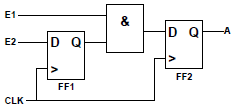
\includegraphics[]{pictures/einfach.png}
\caption{Einfaches Schaltwerk}
\end{figure}

Daraus folgt, dass das zweite Flipflop erst dann getriggert werden darf, wenn das Signal dort sicher
angekommen ist. Es gibt also eine maximale Taktfrequenz, mit der die Schaltung betrieben werden darf.
Diese zu finden ist Aufgabe Ihres Programms. Dazu muss das Programm den l"angsten Signalpfad finden
und dessen Laufzeit berechnen. Die Laufzeit h"angt noch von diversen "Au"seren Einfl"ussen wie Temperatur
und Spannung ab, die Sie ebenfalls ber"ucksichtigen sollen.

\begin{figure}[h]
\centering
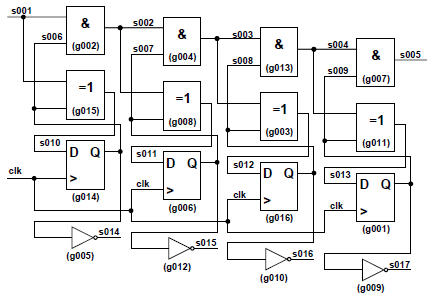
\includegraphics[width=\textwidth]{pictures/rueckwaerts.png}
\caption{R�ckw�rtsz�hler}
\end{figure}

 Dieser stellt im Projektpraktikum das Beispielschaltwerk dar, welches untersucht werden soll.